\documentclass[10pt,a4paper]{article}
%\usepackage[utf8]{inputenc}
\usepackage{fontspec}
\usepackage[polish]{babel}
\usepackage{amsmath}
%\usepackage{amsfonts}
%\usepackage{amssymb}
%\usepackage{makeidx}
%\usepackage{graphicx}
%\usepackage{mathtools}
\usepackage[left=2cm,right=2cm,top=2cm,bottom=2cm]{geometry}
\usepackage[colorlinks]{hyperref}
\usepackage{todonotes}
\usepackage{listings}
\usepackage{graphicx}
\usepackage{float}
\floatstyle{boxed}
\restylefloat{figure}
\usepackage{tikz}
\usepackage[europeanresistors,americaninductors]{circuitikz}



\author{Piotr Miedzik}
\title{MOZA - Projekt 2CAL-A5}
\makeindex
\begin{document}
\maketitle

\listoftodos
\section{Wstęp}
Celem tego projektu było dobranie wzorców pewnego przyrządu pomiarowego, działające w szerokim paśmie częstotliwości, za pomocą metody optymalizacji wielokryterialnej. Do oceny doboru wzorców użyto funkcji:
\[
D(x,f)=|\frac{detM(x,f)}{n+1}|
\]
Co można rozpisać jako:
\[
D = 1-2 |q|^2 - |r|^2 + 2 \cdot Re\left\lbrace s^2 \cdot r^*\right\rbrace
\]
\[
q=\frac{1}{n+1} \sum^n_{k=0}{ e^{j\cdot \cdot \varphi_k}}
\]
\[
r=\frac{1}{n+1} \sum^n_{k=0}{ e^{j\cdot 2\cdot \varphi_k}}
\]
\[
\varphi_k = \frac{4 \cdot \Pi \cdot f}{c} \cdot x_k
\]
\[
c = 3 \cdot e^{8}
\]

Gdzie:\\
$M$ - Macierz Fishera\\
$x$ - zbiór $n$ elementów kalibrujących\\
$f$ - przedział pasma w jakim działa urządzenie\\

Przebieg funkcji $D(x,f)$ można scharakteryzować następującymi parametrami:\\
$r$ - wielkość zafalowań przebiegu w paśmie działa urządzenia\\
$f_L$ - dolna częstotliwość dla której zafalowania nie przekraczają wartości r\\
$f_U$ – gótna częstotliwość dla której zafalowania nie przekraczają wartości r
\todo{ sprawdzić czy $f_U$ dobrze opisane}

Założeniem projektu jest zlezienie takiego wektora wzorców x by zminimalizować wielkość zafalowań $r$ dla $f_U=18GHz$, $f_L=3.6GHz$. Jednocześnie przyjęto ograniczenie że każdy element wektora $x \in \left\langle 0.01;0.2 \right\rangle$.

Zadanie to rozwiązano dwoma metodami za pomocą programu Matlab i wbudowanego w niego Global Optimization Toolbox, z którego użyto algorytmu wielostartowego oraz algorytmu genetycznego.
\subsection{Algorytm genetyczny}
Algorytm ten losuje w każdej iteracji (generacji) zbiór kandydatów na rozwiązanie (populacje). Następnie każda populacja poddawana jest ocenie a następnie selekcji na rozwiązania które pozostają bez zmian oraz takich które poddawane są albo drobnym losowym zmianom (mutacja) albo są krzyżowane z genotypem rodzica (dobrze ocenionego rozwiązania z poprzedniej populacji). Dzięki tym operacją powstaje nowa populacja.  W ten sposób algorytm przeszukuje przestrzeń rozwiązań i podaje najlepsze jakie znalazł.

\subsection{Algorytm wielokartowy}
Algorytm ten szuka rozwiązań dokonując na początku losowania wybranej liczby punktów zawierających się w zadanych granicach, a następnie minimalizuje zadaną funkcję celu przyjmując w kolejnych iteracjach każdy z punktów za punkt startowy. Losowe punkty rozłożone są równomiernie. Każdy punkt startowe optymalizuje funkcję, może jednak natrafić na minimum lokalne, dlatego ze zbioru uzyskanych minimów wybierane jest minimum globalne.

\subsection{nazwać to jakoś}
Jako miary jakości wyniku przyjęto następujące kryteria:
\begin{itemize}
\item Wielkość zafalowań$r$
\item Różnica między przyjętymi czętotliwościami granicznymi($f_L$ i $f_U$) a rzeczywistymi
\item Odchylenie standardowe w paśmie $\left\langle f_L;f_U \right\rangle$.
\item Czas trwania obliczeń
\end{itemize}

\section{Realizacja}

\subsection{Pliki dostarczone przez prowadzącego}
W ramach projektu dostarczone od prowadzącego zostały następujące pliki:

\subsubsection{calc\_D.m}
Funkcja oblicza wartość funkcji D$(x,f)$ oceniającej dobor wzorców która została opisana w poprzednim
punkcie.
\subsubsection{calc\_fLfU.m}
Oblicza wartość $f_L$, $f_U$ oraz najniższą wartość jaką przyjmuje funkcja w tym przedziale z której obliczana jest wielkość zafalowań $r$.

\subsection{Pliki stworzone}
Na potrzeby wykonania zadania stworzono 6 plików:

\subsubsection{Funkcja\_celu.m}
Funkcja celu która wykorzystuje funkcje calc\_D oraz calcfLfU by obliczyć wielkość zafalowań dla
danego wektora wozrców $x$ w zadanym przedziale częstotliwości $f$.

\subsubsection{Freq\_con.m}
Funkcja z ograniczeniami nieliniowymi. Ograniczenia te dotyczły częstotliwości, tzn.
 $f_U=18GHz$, $f_L=3.6GHz$ oraz $D(f_U)=D(f_L)$.
Ograniczenia te okazały się sprawić najwięcej problemów w projekcie.
Wypróbowano różne zestawy ograniczeń, zarówno równościowych jak i nierównościowych.
Ograniczenia równościowe nie dawały żadnych wyników,
solver przerywał wykonywanie algorytmu nie znajdując rozwiązania.
Ograniczenia nierównośćiowe dawały również wyniki niestadyfakcjonujące,
przeważnie z dużymi zafalowaniami (około 0.45).
Dlatego najlepszym rozwiązaniem okazało się dodanie ograniczenia nierównościowego związanego tylko z $D(f_U)=D(f_L)$ oraz dobór odpowiedniego przedział częstotliwości optymalizacji w funkcji celu.
Odpowiedni przedział dobrany został metodą prób i błędów.

\subsubsection{Genetyczny.m}
W tym pliku uruchamiany jest algorytm genetyczny.
Po skończeniu obliczeń środowisko jest zapisywane do pliku genetyczny.mat.
Parametry algorytmu:
\begin{itemize}
\item Liczba zmiennych: 7
\item Populacji: 10000
\item Ograniczenia na populacje początkową: $x \in \left\langle 0.01;0.2 \right\rangle$
\item Ograniczenie dolne i góre wyniku: $x \in \left\langle 0.01;0.2 \right\rangle$
\end{itemize}
\subsubsection{Genetyczny\_wyniki.m}
Plik ładuje wyniki z pliku genetyczny.mat w celu prezentacji wyników

\subsubsection{Multi.m}
W tym pliku uruchamiany jest algorytm wielostartowy.
Po skończeniu obliczeń środowisko jest zapisywane do pliku multi.mat.
Parametry algorytmu:
\begin{itemize}
\item Ilość punktów startowych: 1000
\item Solver: fmincon
\item Rozwiązanie początkowe: $x_k = \frac{k\cdot 3^8}{4 \cdot 18MHz}$
\item Ograniczenie dolne i góre wyniku: $x \in \left\langle 0.01;0.2 \right\rangle$
\end{itemize}
\subsubsection{Multi\_wyniki.m}
Plik ładuje wyniki z pliku genetyczny.mat w celu prezentacji wyników

\section{Wyniki}
Obliczenia wykonywano na komputerze z proceosrem Intel Xeon X5690 @ 3.47GHz, 12GB pamięci RAM z wykorzystaniem pakietu Matlab R2012a w systemie operacyjnym Linux.

najlepsze uzyskane rozwiązania:

\begin{tabular}{|c|c|c|c|c|c|c|c|}
\hline 
 & $x_1$ & $x_2$ & $x_3$ & $x_4$ & $x_5$ & $x_6$ & $x_7$ \\ 
\hline 
Genetyczny & 0.194218 & 0.188177 & 0.157007 & 0.181068 & 0.093069 & 0.197461 & 0.17490 \\ 
\hline 
Multistart & 0.037525 & 0.031646 & 0.024100 & 0.027561 & 0.020383 & 0.016777 & 0.044596 \\ 
\hline 
\end{tabular} 

\begin{figure}[H]
  \caption{Genetyczny}
  \centering
    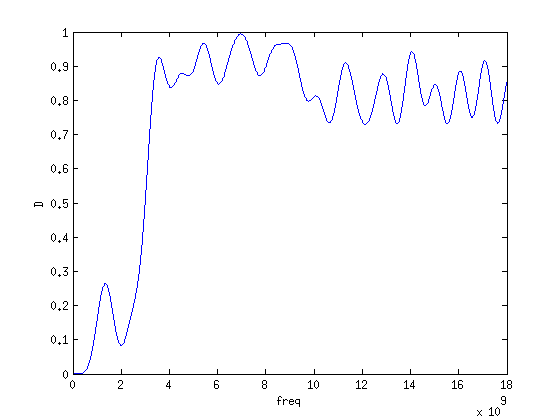
\includegraphics[scale=0.75]{genetyczny}
  \label{fig:genetyczny_wykres}
\end{figure}
\begin{figure}[H]
  \caption{Multistart}
  \centering
    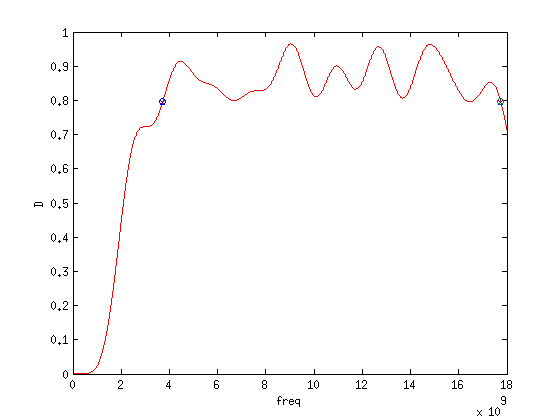
\includegraphics[scale=0.75]{multistart}
  \label{fig:multistart_wykres}
\end{figure}

\begin{tabular}{|c|p{2cm}|p{2cm}|p{2cm}|p{2cm}|p{2cm}|}
\hline 
 & Wielkość \newline zafalowań $r$ & Odchylenie od $f_L$ & Odchylenie od $f_L$ & Odchylenie standardowe w paśmie pracy & Czas \newline obliczeń \\ 
\hline 
Genetyczny & 0.2693 &  5289MHz & 901MHz & 0.0721 & 102s \\ 
\hline 
Multistart & 0.2044 &  124MHz & 251MHz & 0.0488 & 7365s \\ 
\hline 
\end{tabular} 

\vspace{0.5cm}
Optymalizacja przebiegła poprawnie, obydwa algorytmy sprawdziły się.

Algorytm gentyczny wykonywał się szybko w porównaniu do multistartu. Ponieważ algorytm genetyczny polega na losowych zmianach za każdym razem otrzymywany jest inny wynik i trudny do przewidzenia.
Wynik dla algorytmu genetycznego przedstawiony w sprawozdaniu został uzyskany dopiero po kilku próbach. Na rysunku \ref{fig:genetyczny_bad} zostały przedstawione wyniki uzyskane podczas dwuch prób.

Algorytm multistart dał lepszy wynik. Liczbę iteracji ustawiono na 1000 po wcześniejszych próbach z mniejszymi wartościami. W przeciwieństwie do algorytmu genetycznego algorytm multistartu analizuje dużo więcej możliwych rozwiązań, z których wibiera najlepsze. Dzięki temu wyniki algorytm daje nie tylko dużo lepsze wyniki, ale też wynik pod względem jakości za każdym razem jest porównywalny. Algorytm multistartu musi działać niestety znacznie dłużej.

\begin{figure}[H]
  \caption{Wyniki działania algorytmu Genetycznego}
  \centering
    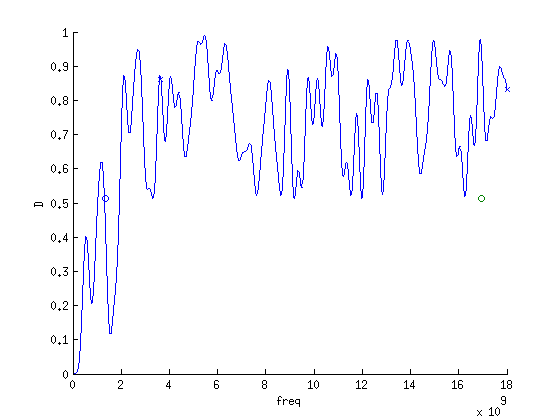
\includegraphics[scale=0.50]{genetyczny_bad}
    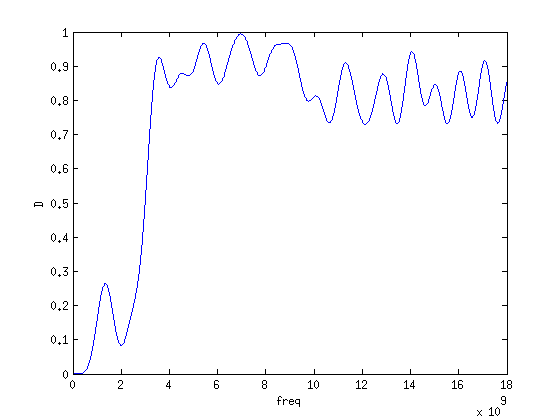
\includegraphics[scale=0.50]{genetyczny}
  \label{fig:genetyczny_bad}
\end{figure}

\subsection{Załączniki}
\begin{itemize}
\item calc\_fLfU.m
\item calc\_D
\item Freq\_con.m
\item Funkcja\_celu.m
\item Genetyczny.m
\item Multi.m
\item Genetyczny\_wyniki.m
\item Multi\_wyniki.m
\end{itemize}
\end{document}